% This must be in the first 5 lines to tell arXiv to use pdfLaTeX, which is strongly recommended.
\pdfoutput=1
% In particular, the hyperref package requires pdfLaTeX in order to break URLs across lines.

\documentclass[11pt]{article}

% Change "review" to "final" to generate the final (sometimes called camera-ready) version.
% Change to "preprint" to generate a non-anonymous version with page numbers.
\usepackage[review]{acl}

% Standard package includes
\usepackage{times}
\usepackage{latexsym}

% For proper rendering and hyphenation of words containing Latin characters (including in bib files)
\usepackage[T1]{fontenc}
% For Vietnamese characters
% \usepackage[T5]{fontenc}
% See https://www.latex-project.org/help/documentation/encguide.pdf for other character sets

% This assumes your files are encoded as UTF8
\usepackage[utf8]{inputenc}

\usepackage{booktabs} % For formal tables
\usepackage{colortbl}
\usepackage{array}
\usepackage{multirow}
\usepackage{ragged2e}
\usepackage{hhline}
\usepackage{hyperref}

% This is not strictly necessary, and may be commented out,
% but it will improve the layout of the manuscript,
% and will typically save some space.
\usepackage{microtype}

% This is also not strictly necessary, and may be commented out.
% However, it will improve the aesthetics of text in
% the typewriter font.
\usepackage{inconsolata}

%Including images in your LaTeX document requires adding
%additional package(s)
\usepackage{graphicx}

% If the title and author information does not fit in the area allocated, uncomment the following
%
%\setlength\titlebox{<dim>}
%
% and set <dim> to something 5cm or larger.

\title{\texttt{ModernAraBERT}: Efficient Adaptation of English Language Models
for Arabic NLP Tasks}

\author{Ahmed Eldamaty \\
Giza Systems \\
Cairo, Egypt \\
\texttt{ahmed.aldamati@gizasystems.com} \\
\And Mohamed Maher \\
University of Tartu \\
Tartu, Estonia \\
\texttt{mohamed.abdelrahman@ut.ee} \\
\And Mohamed Mostafa \\
Giza Systems \\
Cairo, Egypt \\
\texttt{ibrahim.mohamed@gizasystems.com} \\
\And Mariam Ashraf \\
Giza Systems \\
Cairo, Egypt \\
\texttt{mariam.ashraf@gizasystems.com} \\
\And Radwa ElShawi \\
University of Tartu \\
Tartu, Estonia \\
\texttt{radwa.elshawi@ut.ee} \\}

\begin{document}
  \maketitle
  %\begin{abstract}
  %  Transformer-based language models have significantly advanced natural language processing; however, their adaptation to morphologically rich languages like Arabic remains challenging. This paper introduces \texttt{ModernAraBERT}, a resource-efficient approach that effectively adapts an English-pretrained model (\texttt{ModernBERT}) to Arabic NLP tasks. Our methodology involves full pre-training on curated Arabic corpora followed by lightweight fine-tuning on downstream tasks. Comprehensive evaluation in various Arabic NLP tasks, including sentiment analysis, named recognition, and question answering, demonstrates that our approach achieves competitive or superior performance compared to established Arabic models such as \texttt{AraBERT}, with substantially lower computational requirements. Notably, \texttt{ModernAraBERT} shows marked improvements in accuracy for sentiment analysis and named entity recognition tasks, underscoring its strong transfer learning capabilities and broad applicability to Arabic NLP. This framework offers a scalable and effective strategy for extending state-of-the-art language models to Arabic and potentially other underrepresented languages.
  %\end{abstract}

 \begin{abstract}
    Transformer-based language models have significantly advanced natural language processing; however, their adaptation to morphologically rich and dialectally diverse languages such as Arabic remains challenging. This paper introduces \texttt{ModernAraBERT}, a resource-efficient adaptation of the English-pretrained \texttt{ModernBERT} model for Arabic NLP tasks. Our approach combines full pretraining on large-scale curated Arabic corpora with lightweight fine-tuning on downstream benchmarks. We evaluate \texttt{ModernAraBERT} across key Arabic NLP tasks, including sentiment analysis, named entity recognition, and extractive question answering, comparing it against strong baselines~\texttt{AraBERTv1,2}, \texttt{MARBERT}, and \texttt{mBERT}. Experimental results show that \texttt{ModernAraBERT} consistently outperforms all baselines, achieving substantial gains in Macro-F1 and Exact Match scores. These findings highlight the effectiveness of leveraging modern English architectures for efficient cross-lingual adaptation and provide a scalable pathway for extending state-of-the-art transformer models to Arabic and other underrepresented languages.
\end{abstract}


  \section{Introduction}

  %Transformer encoder models such as BERT~\cite{devlin-etal-2019-bert} have revolutionized the approach to language processing tasks, especially within the English language. These models are characterized by their robustness, versatility, and success across numerous NLP applications and language representation tasks~\cite{Gardazi2025}. The Arabic language presents distinctive challenges: it is morphologically rich, replete with inflections, and encompasses various dialects. Consequently, adapting existing models trained on English to Arabic entails unique difficulties~\cite{MATRANE2023101570}.

  %Recent developments in Arabic NLP have been notably driven by the integration of deep learning and transformer-based architectures. The release of \texttt{AraBERT} as a pretrained model for Modern Standard Arabic (MSA) marked the inception of many subsequent Arabic BERT-based models~\cite{antoun2020arabert}. Some focus specifically on MSA, such as \texttt{CAMeLBERT}~\cite{inoue-etal-2021-interplay} and \texttt{ARBERT}~\cite{abdul-mageed-etal-2021-arbert}, which utilized carefully curated data. Others target dialectical variations, including \texttt{MARBERT}~\cite{abdul-mageed-etal-2021-arbert} and \texttt{QARiB}~\cite{abdelali2021pretraining}. However, these initiatives are primarily aimed at developing dedicated Arabic models. Such models, though effective, often incur high computational costs and require training from scratch or extensive adaptation without efficient transfer, or reducing training cost and duplication. Recently, significant advancements have been made through the introduction of \texttt{ModernBERT}~\cite{warner2024modernbert}, which modernizes encoder-only transformer architectures. \texttt{ModernBERT} addresses critical limitations of previous models by training on an extensive dataset of 2 trillion tokens. Its architecture integrates several efficiency and performance improvements, such as rotary positional embeddings (RoPE)~\cite{su2024roformer}, alternating global-local attention layers, and the utilization of GeGLU activation functions~\cite{shazeer2020glu}. These architectural enhancements, combined with a modern tokenizer optimized for diverse textual and code-related data, enable \texttt{ModernBERT} to achieve state-of-the-art performance across a broad spectrum of classification and retrieval tasks, thus providing an optimal foundation for adapting advanced language models to languages with unique linguistic challenges, such as Arabic.

  %The main contributions of this paper can be summarized as follows:
  %\begin{itemize}
   % \item We propose a resource-efficient strategy to extend high-performing English language models to Arabic by conducting comprehensive pretraining on curated Arabic corpora, thus providing a practical alternative by adapting an existing English-pretrained model to Arabic, instead of developing an entirely new Arabic-specific model from scratch.

    %\item We present \texttt{ModernAraBERT}, an adapted version of the state-of-the-art English \texttt{ModernBERT} model, specifically fine-tuned and optimized for Arabic NLP tasks.

    %\item We empirically evaluate \texttt{ModernAraBERT} across three essential Arabic NLP benchmarks: sentiment analysis, named entity recognition, and question answering, demonstrating its superior performance compared to \texttt{AraBERT} baseline. Our approach significantly reduces computational overhead, enhancing accessibility and applicability for research communities and industry practitioners working with Arabic language processing.
 % \end{itemize}










%Transformer encoder models such as BERT~\cite{devlin-etal-2019-bert} have revolutionized natural language processing (NLP), particularly within English. These models exhibit remarkable robustness, versatility, and transferability in numerous NLP applications and representation learning tasks~\cite{Gardazi2025}. However, the Arabic language presents unique challenges: it is morphologically rich, highly inflectional, and characterized by substantial dialectal diversity. Consequently, adapting transformer-based models trained in English to Arabic remains a non-trivial endeavor~\cite{MATRANE2023101570}.
Transformer encoder models such as BERT~\cite{devlin-etal-2019-bert} have transformed natural language processing through their robustness, versatility, and transferability across diverse tasks~\cite{Gardazi2025}. Yet, adapting these models to Arabic remains challenging due to the language’s rich morphology, complex inflection, and extensive dialectal variation~\cite{MATRANE2023101570}.

The rapid progress in Arabic NLP has been driven by the introduction of transformer-based architectures specifically trained or adapted for Arabic. The release of \texttt{AraBERT}~\cite{antoun2020arabert} represented a major milestone, providing the first large-scale pretrained transformer for Modern Standard Arabic (MSA). Its successor, \texttt{AraBERTv2}~\cite{antoun2020arabert}, improved on the original through larger and more diverse pretraining data, enhanced vocabulary coverage, and refined preprocessing for Arabic tokenization. Other models extended this direction by addressing dialectal and social-media variations—most notably \texttt{MARBERT}~\cite{abdul-mageed-etal-2021-arbert}, which was trained primarily on dialectal Arabic tweets, and multilingual baselines such as \texttt{mBERT}~\cite{devlin-etal-2019-bert}, which support Arabic as part of a joint multilingual corpus. While these models have advanced Arabic NLP considerably, they often incur substantial training costs, require specialized data pipelines, and remain limited in efficiently transferring the advances from newer English architectures.

%Recent developments in English transformer encoders, particularly \texttt{ModernBERT}~\cite{warner2024modernbert}, have introduced architectural and efficiency improvements that make large-scale adaptation more feasible. \texttt{ModernBERT} is trained on more than two trillion tokens and incorporates modern design features such as rotary positional embeddings (RoPE)~\cite{su2024roformer}, alternating global-local attention, and GeGLU activation functions~\cite{shazeer2020glu}. These optimizations enable strong performance with significantly improved computational efficiency, making it an ideal foundation for extending high-quality language understanding to morphologically complex languages such as Arabic.
Recent advances in English transformer encoders, particularly \texttt{ModernBERT}~\cite{warner2024modernbert}, have introduced architectural and efficiency enhancements that enable large-scale, cost-effective adaptation. Trained on over two trillion tokens, \texttt{ModernBERT} employs rotary positional embeddings (RoPE)~\cite{su2024roformer}, global-local attention, and GeGLU activations~\cite{shazeer2020glu}, achieving strong performance with high computational efficiency—making it a robust foundation for adapting to morphologically complex languages such as Arabic.


%The main contributions of this paper are as follows.
%\begin{itemize}
  %\item We propose a resource-efficient strategy to adapt a high-performing English model (\texttt{ModernBERT}) to Arabic by conducting a comprehensive pretraining on curated Arabic corpora, providing a practical alternative to developing new Arabic-specific models from scratch.
  
  %\item We introduce \texttt{ModernAraBERT}, an Arabic-adapted variant of \texttt{ModernBERT} optimized for key Arabic NLP tasks.
  
  %\item We empirically evaluated \texttt{ModernAraBERT} in three benchmarks—sentiment analysis, named entity recognition, and question answering against strong baselines including \texttt{AraBERTv1}, \texttt{AraBERTv2}, \texttt{MarBERT}, and \texttt{mBERT}. Our results show consistent and substantial improvements, demonstrating accuracy gains, thereby enhancing the accessibility of advanced transformer architectures for Arabic NLP research and applications.
%\end{itemize}

The main contributions of this paper are as follows.
\begin{itemize}
  \item We propose a resource-efficient strategy for adapting the English \texttt{ModernBERT} model to Arabic through comprehensive pretraining on curated Arabic corpora, offering a practical alternative to developing new Arabic-specific models from scratch.
  
  \item We present \texttt{ModernAraBERT}, an Arabic-adapted variant of \texttt{ModernBERT} optimized for major Arabic NLP tasks.
  
  \item We evaluate \texttt{ModernAraBERT} on sentiment analysis, named entity recognition, and question answering, benchmarking it against \texttt{AraBERTv1}, \texttt{AraBERTv2}, \texttt{MARBERT}, and \texttt{mBERT}. The model consistently outperforms all baselines, demonstrating significant accuracy gains for Arabic NLP research and applications.
\end{itemize}


  \section{Methodology}

  \subsection{Pretraining Corpora}
  For the pretraining phase, we compiled a large-scale Arabic corpus from four publicly available sources: OSIAN~\cite{zeroual-etal-2019-osian}, the Arabic Billion Words dataset~\cite{el20161}, the Arabic Wikipedia dump~\footnote{\href{https://dumps.wikimedia.org/arwiki/}{https://dumps.wikimedia.org/arwiki/}}, and the OSCAR Arabic dataset~\cite{2022arXiv220106642A}. These datasets were chosen to ensure coverage of both Modern Standard Arabic and regional variations. The raw texts were preprocessed through a series of normalization steps, including the removal of special characters, punctuation diacritics, elongation characters, and excess whitespace. To further enhance the morphological quality of the data, we used the Farasa segmenter~\cite{abdelali2016farasa} for affix and root segmentation. The final corpus included over six million sentences, totaling approximately 17~GB in size.

%We extended the original \texttt{ModernBERT} tokenizer, which was trained on English corpora, by adding 80,000 Arabic-specific tokens. The extended vocabulary included segmented roots, inflected forms, and common affixes, ensuring that Arabic morphology was more faithfully captured. Frequent morphological constructions were explicitly added as standalone tokens to improve segmentation consistency and reduce fragmentation.  

%The choice of 80K tokens was empirically validated. As shown in Figure~\ref{fig:vocab}, Arabic follows a long-tailed frequency distribution, where most tokens occur rarely. Our analysis of token frequency (left) and coverage versus vocabulary size (right) demonstrates that coverage improves sharply with vocabulary size but plateaus around 80K tokens. Beyond this point, additional tokens provide negligible coverage gains. Selecting 80K therefore balances corpus coverage with computational efficiency. This cutoff is also consistent with prior Arabic BERT models: \texttt{AraBERT} employs a 64K vocabulary, while \texttt{MARBERT} uses 95K.


\subsection{Tokenization}
We extended the original \texttt{ModernBERT} tokenizer, originally trained on English text, by incorporating 80,000 Arabic-specific tokens. The expanded vocabulary includes segmented roots, inflected forms, and common affixes to better capture Arabic morphology and reduce token fragmentation. The 80K size was selected based on coverage analysis, which showed diminishing returns beyond this threshold, balancing representational adequacy and computational efficiency. This choice also aligns with prior Arabic models, where \texttt{AraBERT} employs a 64K vocabulary and \texttt{MARBERT} uses 95K.


\subsection{Model Training}
Our model is based on the publicly available \texttt{ModernBERT} architecture~\href{https://huggingface.co/answerdotai/ModernBERT-base}{ModernBERT-base} with 22 transformer layers. The embedding layer was resized to accommodate the extended Arabic vocabulary. Pretraining followed the Masked Language Modeling (MLM) objective for three epochs, with sequence lengths of 128 in the first two epochs and 512 in the final epoch to balance efficiency and contextual coverage. The context length was limited to 512 tokens for comparability with baselines like \texttt{AraBERT}. Optimization used AdamW with cosine learning rate decay and gradient clipping. The training progress was tracked via loss and perplexity on a held-out validation set.

The model used in this work is based on the publicly available \texttt{ModernBERT}-base~\footnote{\href{https://huggingface.co/answerdotai/ModernBERT-base}{ModernBert-Base}} architecture as shown in Figure~\ref{fig:model}.


\begin{figure}[h!]
    \centering
    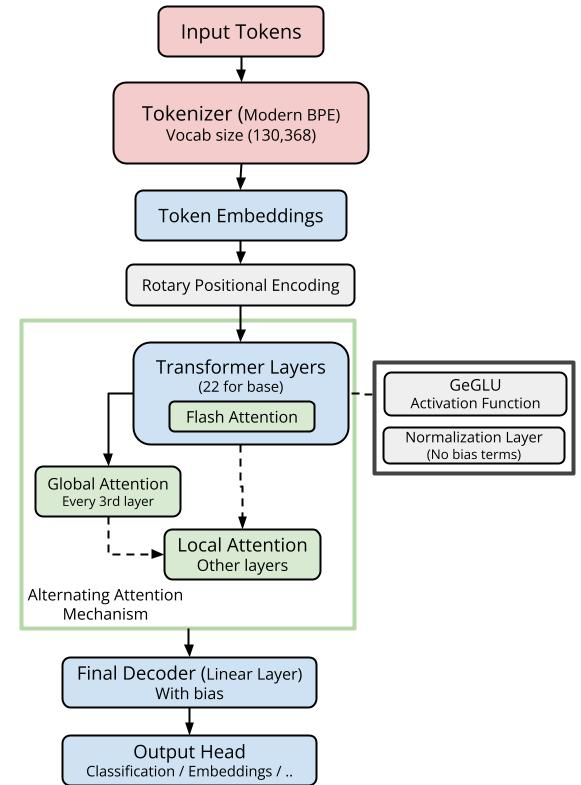
\includegraphics[width=0.4\textwidth]{
      latex/ModernArabert (1).jpg
    } % Replace with your file name
    \caption{ModernBERT Architecture with extended tokenizer vocabulary size and
    embedding layer}
    \label{fig:model}
\end{figure}

Our pretrained \texttt{ModernAraBERT} has been made available~\footnote{\href{http://}{Huggingface URL will be revealed upon review}}. Training and benchmark evaluation scripts are also available in our repository~\footnote{\href{https://anonymous.4open.science/r/ModernAraBERT-823C/}{Our Repository}}.
%https://huggingface.co/gizadatateam/ModernAraBERT
%https://github.com/giza-data-team/ModernAraBERT

\section{Experimental Setup}
All pretraining and fine-tuning were conducted on a high-performance node equipped with 12 CPU cores, 32~GB RAM, and a 40~GB NVIDIA A100 GPU. We evaluated \texttt{ModernAraBERT} on three Arabic NLP tasks: Sentiment Analysis (SA), Named Entity Recognition (NER), and Question Answering (QA). During benchmarking, the pretrained encoder was frozen, and only task-specific classification heads were fine-tuned to reduce training time and overfitting on limited datasets. Each task was trained for up to 200 epochs with an early stopping patience of 10, except NER, which was trained for 5 epochs.


%\paragraph{Sentiment Classification}
%We benchmarked sentiment classification using three datasets:  
%\begin{itemize}
 %   \item \textbf{Hotel Arabic Reviews Dataset (HARD)}~\cite{Elnagar2018}, comprising reviews in both Modern Standard Arabic (MSA) and dialectal Arabic. Following~\cite{antoun2020arabert}, we excluded neutral 3-star reviews, yielding a binary classification setting.  
  %  \item \textbf{Arabic Jordanian General Tweets (AJGT)} Corpus\footnote{\href{https://github.com/komari6/Arabic-twitter-corpus-AJGT}{AJGT Dataset}}, containing 1,800 tweets labeled as positive or negative.  
  %  \item \textbf{Large-Scale Arabic Book Reviews (LABR)}~\cite{aly-atiya-2013-labr}, using the unbalanced binary version for consistency with prior work.  
%\end{itemize}  

%For datasets without predefined splits, we followed a 60/20/20 train/validation/test partition. Sentence-level representations were derived from the \texttt{[CLS]} token and passed to a classification head for binary or multi-class prediction. Performance was measured using Macro F1-score. 

%\paragraph{Named Entity Recognition}
%NER experiments were performed on the ANERCorp dataset~\cite{Benajiba:2007}, using the official CAMeL Lab splits provided via HuggingFace~\cite{obeid2020camel}. The dataset includes entities such as \texttt{Person}, \texttt{Location}, and \texttt{Organization}.  

%We adopted the IOB2 tagging scheme~\cite{Ramshaw1999}. To ensure correct alignment under subword tokenization:  
%- the first subtoken of each word was assigned the gold entity label,  
%- continuation subtokens were either mapped to the corresponding I-label (e.g., \texttt{B-PER} $\rightarrow$ \texttt{I-PER}) if available, or masked with \texttt{-100} during loss computation.  

%This setup ensures entity-level consistency and avoids label fragmentation across subtokens. A token classification head was placed above the encoder, with evaluation reported as macro F1-score at the entity level, following established NER practice.  

%\paragraph{Question Answering}
%For extractive QA, we combined Arabic-SQuAD~\cite{Mozannar:2019} with 50\% of ARCD~\cite{mozannar-etal-2019-neural} as training data, reserving the remaining 50\% of ARCD for testing. This setup provides both coverage and comparability with prior Arabic QA studies.  

%The QA head comprised the pretrained encoder, a prediction layer, and a linear classifier producing start and end span logits. Regularization was applied via dropout (0.1). Hyperparameters included 200 training epochs, AdamW optimizer (learning rate $3\times10^{-5}$), batch sizes of 64 for \texttt{AraBERT} and 32 for \texttt{ModernAraBERT}, and early stopping based on validation F1.  

%Question–context pairs were tokenized to a maximum of 512 tokens with a document stride of 128 for long contexts. Character-level answer spans were mapped to token indices, and cross-entropy loss was computed jointly over start and end positions. During inference, the predicted answer span was extracted by selecting the start–end token pair with maximum joint probability.  Evaluation followed Exact Match (EM) metric, providing complementary measures of exactness.  



\paragraph{Sentiment Classification}
We evaluated sentiment classification on three benchmark datasets. The Hotel Arabic Reviews Dataset (HARD)~\cite{Elnagar2018} contains both Modern Standard Arabic (MSA) and dialectal reviews; following~\cite{antoun2020arabert}, neutral 3-star entries were excluded to form a binary classification setup. The Arabic Jordanian General Tweets (AJGT) corpus\footnote{\href{https://github.com/komari6/Arabic-twitter-corpus-AJGT}{AJGT Dataset}} consists of 1,800 tweets labeled as positive or negative, while the Large-Scale Arabic Book Reviews (LABR) dataset~\cite{aly-atiya-2013-labr} was used in its unbalanced binary version for comparability with prior work. For datasets without predefined splits, we adopted a 60/20/20 train/validation/test partition. Sentence-level representations were obtained from the \texttt{[CLS]} token and passed through a classification head, with performance evaluated using the Macro F1-score.

\paragraph{Named Entity Recognition}
NER experiments were conducted on the ANERCorp dataset~\cite{Benajiba:2007} using the official CAMeL Lab splits~\cite{obeid2020camel}, which include entities such as \texttt{Person}, \texttt{Location}, and \texttt{Organization}. The IOB2 tagging scheme~\cite{Ramshaw1999} was employed, assigning the gold entity label to the first subtoken of each word, while continuation subtokens were mapped to the corresponding I-label or masked with \texttt{-100} during loss computation. A token classification head was placed on top of the encoder, and results were reported as entity-level macro F1-scores, following standard NER evaluation practice.

\paragraph{Question Answering}
For extractive question answering, we combined Arabic-SQuAD~\cite{Mozannar:2019} with 50\% of ARCD~\cite{mozannar-etal-2019-neural} for training and reserved the remaining ARCD data for testing. The model architecture included the pretrained encoder, a prediction layer, and a linear classifier for start and end span logits. Training employed AdamW (learning rate $3\times10^{-5}$) with dropout (0.1), a maximum of 200 epochs, and early stopping based on validation F1. Inputs were tokenized to a maximum length of 512 with a document stride of 128, and character-level answer spans were aligned with token indices. Cross-entropy loss was computed jointly over start and end positions, and during inference, the span with the highest joint probability was selected. Evaluation was performed using the Exact Match (EM) metric.




\section{Results and Discussion}

%\subsection{Sentiment Classification}
%Table~\ref{tab:sentiment_results} presents the SA accuracy results for our adapted \texttt{ModernAraBERT} compared to the \texttt{AraBERT} baseline. \texttt{ModernAraBERT} outperforms the baseline AraBERT at all datasets despite only training the prediction head. This suggests that the features learned during pre-training on Arabic data were effectively transferred.
\subsection{Sentiment Classification}
Table~\ref{tab:sentiment_results} reports the Macro-F1 scores for sentiment classification across the LABR, HARD, and AJGT datasets. \texttt{ModernAraBERT} achieves the best performance on all three benchmarks, surpassing prior Arabic models by a substantial margin. Specifically, it improves over the most widely adopted baseline (\texttt{AraBERTv1}) by +11\% on LABR, +16\% on HARD, and +12\% on AJGT. Notably, while \texttt{mBERT} and \texttt{MARBERT} perform competitively on AJGT, they lag considerably on MSA-heavy datasets such as LABR and HARD. These results indicate that the pretraining of \texttt{ModernAraBERT} on large-scale Arabic corpora captures both standard and dialectal features effectively, yielding robust transfer across diverse sentiment domains despite limited fine-tuning.


\begin{table}[ht]
    \centering
    \small % or \footnotesize if needed
    \caption{Macro-F1 (\%) comparison of \texttt{ModernAraBERT} and other Arabic language models across sentiment datasets. Best scores per dataset are in bold.}
    \label{tab:sentiment_results}
    \begin{tabular}{l@{\hspace{0.4cm}}c@{\hspace{0.4cm}}c@{\hspace{0.4cm}}c}
        \toprule
        \textbf{Model} & \textbf{LABR} & \textbf{HARD} & \textbf{AJGT} \\
        \midrule
        AraBERTv1 & 45.35 & 72.65 & 58.01 \\
        AraBERTv2 & 45.79 & 67.10 & 53.59 \\
        mBERT     & 44.18 & 71.70 & 61.55 \\
        MARBERT   & 45.54 & 67.39 & 60.63 \\
        \textbf{ModernAraBERT} & \textbf{56.45} & \textbf{89.37} & \textbf{70.54} \\
        \bottomrule
    \end{tabular}\\
    \vspace{0.1cm}
\end{table}


\subsection{Named Entity Recognition (NER)}
\label{sec:ner_results}
Table~\ref{tab:ner_results} presents the Macro-F1 results for the NER task. \texttt{ModernAraBERT} achieves a clear improvement over all baselines, reaching 28.23\% compared to 16.77\% for \texttt{AraBERTv2} and 13.46\% for \texttt{AraBERTv1}. This represents a relative gain of over 68\% against the strongest prior Arabic model. The performance gap is even larger when compared to \texttt{mBERT} and \texttt{MARBERT}, which struggle to generalize beyond domain-specific training. These results highlight the ability of \texttt{ModernAraBERT} to learn richer token-level representations that effectively capture Arabic morphological and contextual cues, improving entity boundary detection despite limited fine-tuning.

\begin{table}[ht]
    \centering
    \small % or \footnotesize if needed
    \caption{Macro-F1 (\%) comparison of \texttt{ModernAraBERT} and other models on the NER task. Best score is in bold.}
    \label{tab:ner_results}
    \begin{tabular}{l@{\hspace{0.4cm}}c}
        \toprule
        \textbf{Model} & \textbf{NER (Macro-F1)} \\
        \midrule
        AraBERTv1   & 13.46 \\
        AraBERTv2   & 16.77 \\
        mBERT       & 12.15 \\
        MARBERT     & 7.42  \\
        \textbf{ModernAraBERT} & \textbf{28.23} \\
        \bottomrule
    \end{tabular}\\
    \vspace{0.1cm}
\end{table}


\subsection{Question Answering}
Table~\ref{tab:qa_results} presents the Exact Match (EM) results on the ARCD test split. \texttt{ModernAraBERT} achieves the highest EM score of 27.10\%, outperforming all baselines including \texttt{AraBERTv2} (26.08\%), \texttt{AraBERT} (25.36\%), \texttt{mBERT} (25.12\%), and \texttt{MARBERT} (23.58\%). Although the absolute gains appear moderate, they are consistent across all baselines, demonstrating the effectiveness of the adapted model in capturing precise answer spans. The improvements indicate that pretraining on large-scale Arabic corpora enhances contextual understanding and span localization, enabling \texttt{ModernAraBERT} to better align question and context representations in extractive QA tasks.

\begin{table}[ht]
    \centering
    \small
    \caption{Extractive Question Answering Results (Exact Match, \%) on \texttt{ARCD} Test Split.}
    \label{tab:qa_results}
    \begin{tabular}{l@{\hspace{0.4cm}}c}
        \toprule
        \textbf{Model} & \textbf{EM} \\
        \midrule
        AraBERT     & 25.36 \\
        AraBERTv2   & 26.08 \\
        mBERT       & 25.12 \\
        MARBERT   & 23.58 \\
        \textbf{ModernAraBERT} & \textbf{27.10} \\
        \bottomrule
    \end{tabular}\\
    \vspace{0.1cm}
    \footnotesize \textit{EM: Exact Match.}
\end{table}


\subsection{Overall Analysis}
Across all evaluated NLP tasks, adapting an English-pretrained model like \texttt{ModernAraBERT} to Arabic through our two-phase approach with complete pretraining followed by lightweight fine-tuning of task-specific heads yielded consistently strong performance. The model outperformed \texttt{AraBERTv1}, \texttt{AraBERTv2}, \texttt{MARBERT}, and \texttt{mBERT} baselines, with the most notable gains observed in NER and QA. These results demonstrate the effectiveness of leveraging large-scale English architectures for Arabic transfer learning while maintaining reasonable computational efficiency. 

%\subsection{Hardware Resource Usage}
% our comparison of computational efficiency during the NLP tasks benchmarking revealed trade-offs between the models. Table~\ref{tab:hardware_usage} summarizes memory consumption across models and tasks during head training. Overall, \texttt{AraBERT} remained the most memory-efficient model, showing the lowest RAM and VRAM usage across benchmarks. In contrast, \texttt{ModernAraBERT} required higher resources, particularly in QA (5.90~GB RAM, 20.84~GB VRAM) and SA (9.85~GB RAM, 20.63~GB VRAM), reflecting the increased parameter footprint introduced by the extended Arabic vocabulary and larger architecture. Nevertheless, this higher computational cost was accompanied by substantial performance improvements across all tasks. The observed trade-off suggests that while \texttt{AraBERT} remains advantageous for memory-constrained or latency-critical environments, \texttt{ModernAraBERT} provides a better balance of accuracy and resource utilization for high performance Arabic NLP applications.

\subsection{Hardware Resource Usage}
Beyond accuracy, Table~\ref{tab:hardware_usage} summarizes memory consumption across models during head training. \texttt{AraBERT} was the most memory-efficient, showing the lowest RAM and VRAM usage across all tasks, while \texttt{ModernAraBERT} required more resources particularly in QA (5.90~GB RAM, 20.84~GB VRAM) and SA (9.85~GB RAM, 20.63~GB VRAM) due to its larger architecture and extended vocabulary. This increase in computational cost was offset by consistent performance gains, indicating that \texttt{ModernAraBERT} offers a favorable trade-off between accuracy and resource utilization, whereas \texttt{AraBERT} remains better suited for memory-constrained or latency-sensitive scenarios.

\begin{table}[ht]
    \centering
    \small
    \caption{Hardware Resource Usage Across Models and Benchmarks (Memory usage in GB)}
    \label{tab:hardware_usage}
    \begin{tabular}{l@{\hspace{0.25cm}}l@{\hspace{0.25cm}}c@{\hspace{0.25cm}}c}
        \toprule 
        \textbf{Benchmark} & \textbf{Model} & \textbf{Peak RAM} & \textbf{Peak VRAM} \\
        \midrule 
        \multirow{3}{*}{QA} & AraBERT & 4.52 & 13.50 \\
                             & mBERT & 1.57 & 13.66 \\
                             & MARBERT & 1.93 & 13.60 \\
                             & ModernAraBERT & 5.90 & 20.84 \\
        \hline
        \multirow{3}{*}{NER} & AraBERT & 5.55 & 6.95 \\
                            & mBERT & 4.85 & 7.91 \\
                            & MARBERT & 7.76 & 7.40 \\
                            & ModernAraBERT & 6.49 & 10.42 \\
        \hline
        \multirow{3}{*}{SA} & AraBERT & 8.34 & 13.50 \\
                            & mBERT & 8.36 & 13.66 \\
                            & MARBERT & 8.28 & 13.61 \\
                            & ModernAraBERT & 9.85 & 20.63 \\
        \bottomrule
    \end{tabular}
\end{table}

\section{Conclusion}
In this paper, we introduced \texttt{ModernAraBERT}, a resource-efficient adaptation of the English \texttt{ModernBERT} model for Arabic NLP. By fully pretraining on large-scale Arabic corpora and fine-tuning on downstream tasks, \texttt{ModernAraBERT} achieved consistent gains across sentiment analysis, named entity recognition, and question answering benchmarks. It outperformed strong baselines \texttt{AraBERT}, \texttt{MARBERT}, and \texttt{mBERT} with Macro-F1 improvements exceeding 10\% in sentiment analysis, more than doubling NER performance, and yielding the highest Exact Match score in QA. These results demonstrate that modern English architectures can be efficiently transferred to morphologically rich languages, providing a scalable framework for extending state-of-the-art transformer models to Arabic and other underrepresented languages.

\section{Limitations}
While \texttt{ModernAraBERT} demonstrates consistent improvements across SA, NER, and QA benchmarks, several limitations remain.  

First, the adaptation approach focuses on full pretraining followed by head-only fine-tuning. While computationally efficient, this design limits deeper task-specific optimization of the encoder, which may constrain performance in tasks requiring fine-grained reasoning.  

Second, the model relies on the Byte-BPE (BBPE) tokenizer used in \texttt{ModernBERT}, which differs from the WordPiece tokenizers employed by most Arabic BERT variants such as \texttt{AraBERT} and \texttt{MARBERT}. Recent findings~\cite{qarah2024comprehensive} indicate that BBPE-based models can underperform on extractive QA tasks compared to WordPiece or SentencePiece-based counterparts, particularly when precise span alignment is required. This may explain the relatively smaller performance gain observed for \texttt{ModernAraBERT} on the ARCD dataset compared to its stronger improvements in SA and NER tasks.  

Finally, although the experiments cover key Arabic NLP tasks, broader evaluation on additional downstream applications and dialectal datasets would provide a more comprehensive assessment of generalization. Future work will explore tokenizer adaptations and selective layer fine-tuning to further enhance cross-task robustness.



%\section*{Acknowledgments}
%This work was supported by the project "Increasing the knowledge intensity of Ida-Viru entrepreneurship" co-funded by the European Union and the innovation hub at Giza Systems~\footnote{https://gizasystems.com}.

  % Bibliography entries for the entire Anthology, followed by custom entries
  %\bibliography{anthology,custom}
  % Custom bibliography entries only
  \bibliography{custom}

  %\appendix

  %\section{Example Appendix}
  %\label{sec:appendix}

  %This is an appendix.
\end{document}